\documentclass[12pt, twoside]{article}
\usepackage[letterpaper, margin=1in, headsep=0.5in]{geometry}
\usepackage[english]{babel}
\usepackage[utf8]{inputenc}
\usepackage{amsmath}
\usepackage{amsfonts}
\usepackage{amssymb}
\usepackage{tikz}
\usetikzlibrary{quotes, angles}
\usepackage{graphicx}
\usepackage{enumitem}
\usepackage{multicol}

\newif\ifmeta
\metatrue %print standards and topics tags

\title{Regents Geometry}
\author{Chris Huson}
\date{January 2022}

\usepackage{fancyhdr}
\pagestyle{fancy}
\fancyhf{}
\renewcommand{\headrulewidth}{0pt} % disable the underline of the header
\raggedbottom

\fancyhead[LE]{\thepage}
\fancyhead[RO]{\thepage \\ Name: \hspace{4cm} \,\\}
\fancyhead[LO]{BECA / Dr. Huson / Geometry 6 Trigonometry}

\begin{document}

\subsubsection*{6.6 Classwork: Tangent inverse \hfill CCSS.HSG.SRT.C.8}
\begin{enumerate}
  \item \begin{enumerate}
    \item Do Now: Graph and label $\triangle ABC$ with $A(0,0)$, $B(6,8)$, and $C(6,0)$.
    \begin{center}
      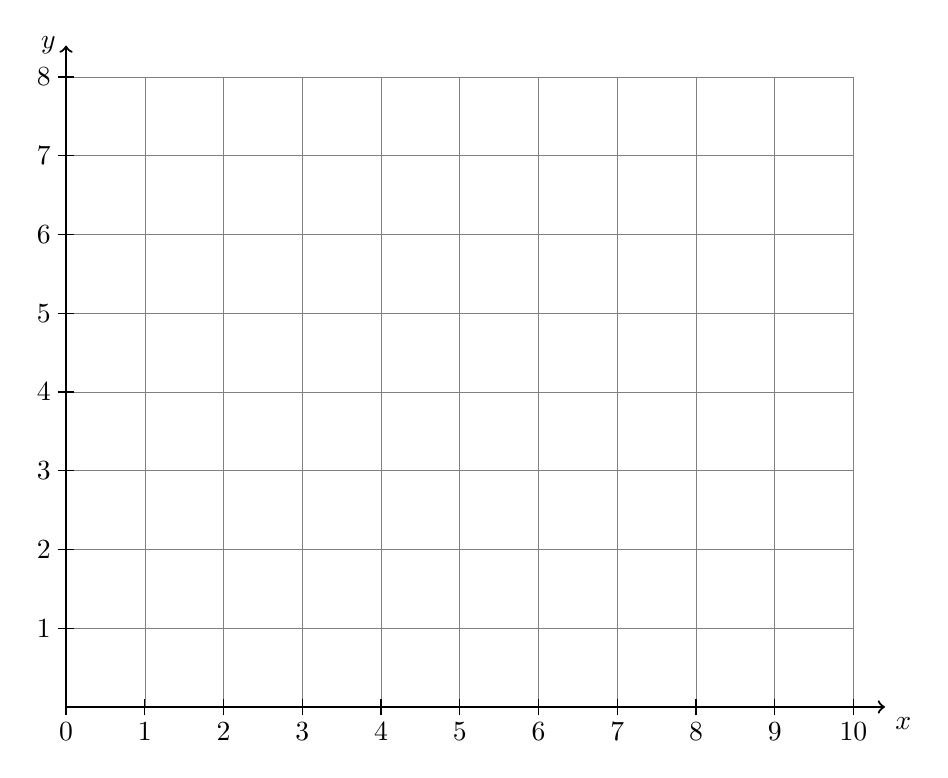
\begin{tikzpicture}
        \draw [help lines] (0,0) grid (10,8);
        \draw [thick, ->] (0,0) -- (10.4,0) node [below right] {$x$};
        \draw [thick, ->] (0,0)--(0,8.4) node [left] {$y$};
        \foreach \x in {0,1,...,10}
        \draw[shift={(\x,0)},color=black] (0pt,-3pt) -- (0pt,3pt) node[below=5pt]  {$\x$};
      \foreach \y in {1,2,3,4,5,6,7,8}
        \draw[shift={(0,\y)},color=black] (-3pt,0pt) -- (3pt,0pt) node[left=5pt]  {$\y$};
      \end{tikzpicture}
    \end{center}
    \item Find the lengths of the sides of $\triangle ABC$.
    \begin{multicols}{2}
      $AC=$ \hspace{3cm}
      $BC=$ \\[1cm]
      $AB=\sqrt{AC^2+BC^2}$
    \end{multicols} \vspace{2.5cm}
    \item Find the slope and $y$-intercept of the line $\overleftrightarrow{AB}$.
      \begin{multicols}{2}
        $m_{AB}=$ \\
        $b_{AB}=$
      \end{multicols} \vspace{0.25cm}
    \item Write down the equation of each line. \\[0.5cm]
      $\overleftrightarrow{AB}$: \hfill
      $\overleftrightarrow{BC}$: \hfill
      $\overleftrightarrow{AC}$: \hspace{2cm}
    \vspace{1cm}
    \item Find the measure of $\angle BAC=\theta$ in degrees with a protractor. \vspace{0.5cm}
    \item Find the slope of $\overleftrightarrow{AB}$ using the tangent function.\\[0.5cm]
    $\displaystyle \tan(\theta)=$
  \end{enumerate}

\newpage
\item Use a calculator. Complete the table mapping angle measures to slope. \vspace{0.25cm}
\begin{multicols}{2}
  \begin{enumerate}
    \item $\tan 15^\circ = $
    \item $\tan 30^\circ =$
    \item $\tan 45^\circ = $
    \item $\tan 60^\circ =$
    \item $\tan 75^\circ = $
    \item $\tan 90^\circ =$
  \end{enumerate}
  \begin{tabular}{l|r}
    angle $\theta$ & $\tan(\theta)$\\
    \hline
    0 & 0 \\[0.25cm]
    $15^\circ$ & \\[4cm]
  \end{tabular}
\end{multicols} \vspace{0.5cm}

\item Complete the table. Use the Pythagorean theorem, $a^2+b^2=c^2$, and your table in \#2.
\begin{center}
  \begin{tabular}{c|c|c|c}
    coordinate pair $(x,y)$ & hypotenuse ($c$) & slope ($m$) & angle $\theta$\\
    \hline
    $(24,7)$ & 25  & $0.29...$ & $16^\circ$\\[0.25cm]
    $(15,8)$ & 17  & $0.5\overline{3}$ & $28^\circ$\\[0.5cm]
    $(4,3)$ &  &  & \\[0.5cm]
    $(6,8)$ &  &  & \\[0.5cm]
    $(5,12)$ &  &  & 
  \end{tabular}
\end{center}
  \begin{tikzpicture}[scale=0.5]
    %\draw [help lines] (0,0) grid (25,13);
    \draw [thick, ->] (0,0) -- (25.8,0) node [right] {$x$};
    \draw [thick, ->] (0,0)--(0,15.8) node [right] {$y$};
    \foreach \x in {0,5,...,25}
      \draw[shift={(\x,0)},color=black] (0pt,-3pt) -- (0pt,3pt) node[below=5pt]  {$\x$};
    \foreach \y in {5,10,15}
      \draw[shift={(0,\y)},color=black] (-3pt,0pt) -- (3pt,0pt) node[left=5pt]  {$\y$};
    \draw [dashed] (0:25) arc (0:20:25);
    \draw [dashed, line width=1pt, ->] (0,0)--(24,7);
    \draw [fill] (4,3) circle [radius=0.1cm] node[above right]{$(4,3)$};
    \draw [fill] (5,12) circle [radius=0.1cm] node[above]{$(5,12)$};
    \draw [fill] (6,8) circle [radius=0.1cm] node[above right]{$(6,8)$};
    \draw [fill] (24,7) circle [radius=0.1cm] node[above right]{$(24,7)$};
    \draw [fill] (15,8) circle [radius=0.1cm] node[above right]{$(15,8)$};
  \end{tikzpicture}

\newpage
\subsubsection*{Definitions and vocabulary}
Right triangle $\triangle ABC$ with side lengths $a$, $b$, $c$. $m\angle A = \theta$
  \begin{center}
  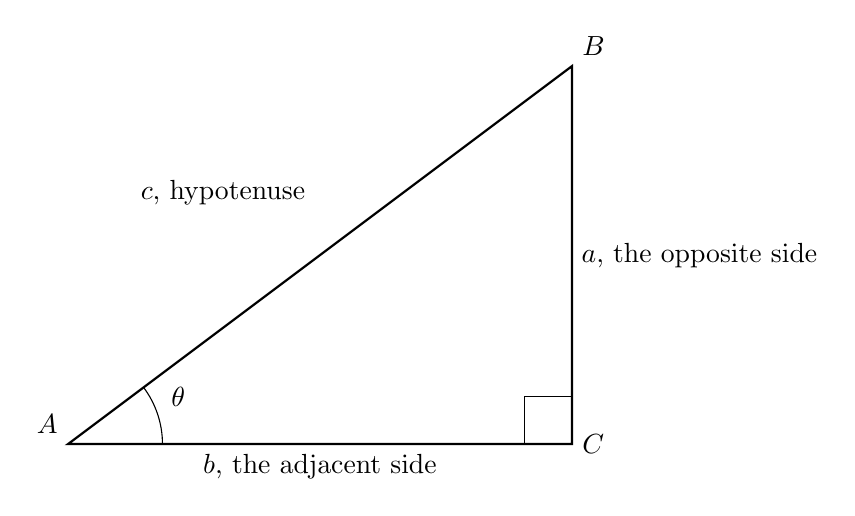
\begin{tikzpicture}[scale=0.8]
    \draw [thick](0,0)node[above left]{$A$}--
        (8,0)node[right]{$C$}--
        (8,6)node[above right]{$B$}--cycle;
    \node at (1.75,0.75){$\theta$};
    \draw (1.5,0) arc (0:37:1.5);
    \draw (8,0) ++(-0.75,0)--+(0,0.75)--+(0.75,0.75);
    \node at (4,0) [below]{$b$, the adjacent side};
    \node at (8,3) [right]{$a$, the opposite side};
    \node at (1,4) [right]{$c$, hypotenuse};
  \end{tikzpicture}
  \end{center}

A \emph{Pythagorean triple} is a set of three positive integers that 
satisfies $a^2+b^2=c^2$. They comprise the side lengths of a right triangle.\\[1cm]
The \emph{tangent} function maps angle measures onto slope, rise over run, or opposite over adjacent.
\begin{center}
$\displaystyle \tan(\theta)=\frac{opposite}{adjacent}$
\end{center}
The \emph{inverse tangent} function maps slope onto angle measure. It is the opposite of the tangent function.
\begin{center}
$\displaystyle \tan^{-1}\left(\frac{opposite}{adjacent}\right)=\theta$
\end{center}
The most common units of angle measures are degrees, radians, and grads.\begin{center}
\begin{tabular}{lcc}
  Unit & full turn & quarter turn\\[0.1cm]
  \hline\\
  degrees & $360^\circ$ & $90^\circ$\\[0.25cm]
  radians & $2\pi$ & $\displaystyle \frac{\pi}{2}$\\[0.35cm]
  grads & 400 & 100
\end{tabular}
\end{center}
Convert radians to degrees with the formula
\begin{center}
 $\pi \, \rm{radians}=180^\circ$
\end{center}

\end{enumerate}
\end{document}
